\documentclass[12pt]{article}
\usepackage{pylatex}
\usepackage{mpllatex}
\usepackage{geometry}
\usepackage{pgf}
\usepackage{amsmath}
\usepackage{listings}
\usepackage{hyperref}
\usepackage{breqn}
\usepackage{caption}
\usepackage{examples}

\geometry{papersize={210mm,297mm},hmargin=2cm,tmargin=1.0cm,bmargin=1.5cm}

\def\pyLaTeX{{\tt\small pyLaTeX}}
\def\mplLaTeX{{\tt\small mplLaTeX}}

\begin{document}

\section*{Using output from other sources}

This document performs no computations (i.e., it has no active code blocks) but instead uses selected parts of the output created by other documents. Thus this document can be compiled using {\tt\small pdflatex summary}. The basic structure of this document is as follows.

\begin{minipage}[t]{0.75\textwidth}
\begin{latex}
   \documentclass[12pt]{article}
   \usepackage{pylatex}    % so that we can use \py{foo}
   \usepackage{mpllatex}   % so that we can use \mpl{bah}
   \usepackage{amsmath}
   ...                     % other packages such as geometry, hyperref, breqn etc.
   \begin{document}
      ...
      \documentclass[12pt]{mpllatex}
\usepackage{examples}

\begin{document}

\section*{Elementary maths}

\begin{maple}
   ans := expand((a+b)^3):                                  # mpl (ans.101,ans)
   ans := factor(-2*x+2*x+a*x-x^2+a*x^2-x^3):               # mpl (ans.102,ans)
   ans := {solve(x^2-4 = 0,x)}:                             # mpl (ans.103,ans) {...} avoids maple/latex syntax error
   sol := solve(x^2-4 = 0,x):                               # multiple roots, can't use mpl(foo,bah) here
   ans := {x=sol[1],x=sol[2]}:                              # mpl (ans.104,ans) fixes problem of multiple roots
   ans := solve({2*a-b = 3, a+b+c = 1,-b+c = 6},{a,b,c}):   # mpl (ans.105,ans)
   ans := evalf[50](Pi):                                    # mpl (ans.106,ans)
   ans := convert(1/((1 + x)*(5 + x)),parfrac):             # mpl (ans.107,ans)
   ans := simplify((1/(1 + x) - 1/(5 + x))/4):              # mpl (ans.108,ans)
   ans := simplify(tanh(ln(x))):                            # mpl (ans.109,ans)
   ans := simplify(tanh(I*x)):                              # mpl (ans.110,ans)
   ans := simplify(sinh(3*x) - 3*sinh(x) - 4*(sinh(x))^3):  # mpl (ans.111,ans)
   ans := ''tanh(ln(x))'':                                  # mpl (lhs.109,ans)
   ans := ''tanh(I*x)'':                                    # mpl (lhs.110,ans)
   ans := ''sinh(3*x) - 3*sinh(x) - 4*(sinh(x))^3'':        # mpl (lhs.111,ans)
\end{maple}

\begin{minipage}[t]{0.65\textwidth}
\begin{align*}
   &\mpl*{ans.101}\\
   &\mpl*{ans.102}\\
   &\mpl*{ans.103}\\
   &\mpl*{ans.104}\\
   &\mpl*{ans.105}\\
   &\mpl*{ans.106}\\
   &\mpl*{ans.107}\\
   &\mpl*{ans.108}\\
   \mpl{lhs.109} &= \Mpl{ans.109}\\
   \mpl{lhs.110} &= \Mpl{ans.110}\\
   \mpl{ans.111} &= \Mpl{lhs.111}
\end{align*}
\end{minipage}
\hskip 1cm
\lower16pt\hbox{%
\begin{minipage}[t]{0.35\textwidth}
\begin{latex}
   \begin{align*}
      &\mpl*{ans.101}\\
      &\mpl*{ans.102}\\
      &\mpl*{ans.103}\\
      &\mpl*{ans.104}\\
      &\mpl*{ans.105}\\
      &\mpl*{ans.106}\\
      &\mpl*{ans.107}\\
      &\mpl*{ans.108}\\
      \mpl{lhs.109} &= \Mpl{ans.109}\\
      \mpl{lhs.110} &= \Mpl{ans.110}\\
      \mpl{ans.111} &= \Mpl{lhs.111}
   \end{align*}
\end{latex}
\end{minipage}}

\clearpage

\section*{Linear Algebra}

\begin{minipage}[t]{0.65\textwidth}
\begin{maple}
   with(LinearAlgebra):
   mat  := <<2|3>, <5|4>>:                        # mpl (ans.201,mat)
   ans  := Eigenvectors(mat,output='list'):
   eig1 := ans[1][1]:                             # 1st eigenvalue
   eig2 := ans[2][1]:                             # 2nd eigenvalue
   v1   := ans[1][3][1]:                          # 1st eigenvector
   v2   := ans[2][3][1]:                          # 2nd eigenvector
   eig  := <eig1,eig2>:                           # mpl (ans.202,eig)
   ans  := <v1|v2>:                               # mpl (ans.203,ans)
   ans  := CharacteristicPolynomial(mat,lambda):  # mpl (ans.204,ans)
   vec  := <3,7>:                                 # mpl (ans.205,vec)
   sol  := LinearSolve(mat,vec):                  # mpl (ans.206,sol)
\end{maple}
\end{minipage}
\hskip 1cm
\begin{minipage}[t]{0.35\textwidth}
\begin{latex}
   \begin{align*}
      &\mpl*{ans.201}\\
      &\mpl*{ans.202}\\
      &\mpl*{ans.203}\\
      &\mpl*{ans.204}\\
      &\mpl*{ans.205}\\
      &\mpl*{ans.206}
   \end{align*}
\end{latex}
\end{minipage}

\begin{align*}
   &\mpl*{ans.201}\\
   &\mpl*{ans.202}\\
   &\mpl*{ans.203}\\
   &\mpl*{ans.204}\\
   &\mpl*{ans.205}\\
   &\mpl*{ans.206}
\end{align*}

\clearpage

\section*{Limits}

\begin{minipage}[t]{0.65\textwidth}
\begin{maple}
   ans := limit(sin(4*x)/x,x=0):                  # mpl (ans.301,ans)
   ans := limit(2^x/x,x=infinity):                # mpl (ans.302,ans)
   ans := limit(((x+dx)^2 - x^2)/dx, dx=0):       # mpl (ans.303,ans)
   ans := limit((4*n + 1)/(3*n - 1),n=infinity):  # mpl (ans.304,ans)
   ans := limit((1+(a/n))^n,n=infinity):          # mpl (ans.305,ans)
\end{maple}
\end{minipage}
\hskip 1cm
\begin{minipage}[t]{0.35\textwidth}
\begin{latex}
   \begin{align*}
      &\mpl*{ans.301}\\
      &\mpl*{ans.302}\\
      &\mpl*{ans.303}\\
      &\mpl*{ans.304}\\
      &\mpl*{ans.305}
   \end{align*}
\end{latex}
\end{minipage}

\vspace{-10pt}

\begin{align*}
   &\mpl*{ans.301}\\
   &\mpl*{ans.302}\\
   &\mpl*{ans.303}\\
   &\mpl*{ans.304}\\
   &\mpl*{ans.305}
\end{align*}

\section*{Series}

\begin{minipage}[t]{0.65\textwidth}
\begin{maple}
   ans := series((1 + x)^(-2), x=1, 6):          # mpl (ans.401,ans)
   ans := series(exp(x), x=0, 6):                # mpl (ans.402,ans)
   ans := sum(1/n^2, n=1..50):                   # mpl (ans.403,ans)
   ans := sum(1/n^4, n=1..infinity):             # mpl (ans.404,ans)
\end{maple}
\end{minipage}
\hskip 1cm
\begin{minipage}[t]{0.35\textwidth}
\begin{latex}
   \begin{align*}
      &\mpl*{ans.401}\\
      &\mpl*{ans.402}\\
      &\mpl*{ans.403}\\
      &\mpl*{ans.404}
   \end{align*}
\end{latex}
\end{minipage}

\begin{align*}
   &\mpl*{ans.401}\\
   &\mpl*{ans.402}\\
   &\mpl*{ans.403}\\
   &\mpl*{ans.404}
\end{align*}

\clearpage

\section*{Calculus}

\begin{minipage}[t]{0.65\textwidth}
\begin{maple}
   ans := diff(x*sin(x),x):                          # mpl (ans.501,ans)
   ans := eval(diff(x*sin(x),x),x=Pi/4):             # mpl (ans.502,ans)
   ans := int(2*sin(x)^2, x=a..b):                   # mpl (ans.503,ans)
   ans := int(2*exp(-x^2),x=0..infinity):            # mpl (ans.504,ans)
   ans := ''int(2*exp(-x^2),x=0..infinity)'':        # mpl (lhs.504,ans)
   ans := int(int(x^2 + y^2,  y=0..x),x=0..1):       # mpl (ans.505,ans)
   ans := ''int(int(x^2 + y^2,  y=0..x),x=0..1)'':   # mpl (lhs.505,ans)
\end{maple}
\end{minipage}
\hskip 1cm
\begin{minipage}[t]{0.35\textwidth}
\begin{latex}
   \begin{align*}
      &\mpl*{ans.501}\\
      &\mpl*{ans.502}\\
      &\mpl*{ans.503}\\
      \mpl{lhs.504}&=\Mpl{ans.504}\\
      \mpl{lhs.505}&=\Mpl{ans.505}
   \end{align*}
\end{latex}
\end{minipage}

\begin{align*}
   &\mpl*{ans.501}\\
   &\mpl*{ans.502}\\
   &\mpl*{ans.503}\\
   \mpl{lhs.504}&=\Mpl{ans.504}\\
   \mpl{lhs.505}&=\Mpl{ans.505}
\end{align*}

\clearpage

\section*{Differential equations}

\begin{minipage}[t]{0.65\textwidth}
\begin{maple}
   ode := diff(y(x),x) + y(x) = 2*a*sin(x):
   ics := y(0) = 0:
   ans := rhs(dsolve(ode)):                    # mpl (ans.601,ans)
   ans := rhs(dsolve([ics,ode])):              # mpl (ans.602,ans)

   ode := diff(y(x),x,x) + y(x) = 0:
   ics := y(0)=0, (D(y))(0) = 1:
   ans := rhs(dsolve(ode)):                    # mpl (ans.603,ans)
   ans := rhs(dsolve([ics,ode])):              # mpl (ans.604,ans)

   ode := diff(y(x),x,x) + 5*diff(y(x),x) - 6*y(x) = 0:
   ans := rhs(dsolve(ode)):                    # mpl (ans.605,ans)
   sol := eval(ans,[_C1=2,_C2=3]):             # mpl (ans.606,sol)
\end{maple}
\end{minipage}
\hskip 1cm
\begin{minipage}[t]{0.35\textwidth}
\begin{latex}
   \begin{align*}
      &\mpl*{ans.601}\\
      &\mpl*{ans.602}\\
      &\mpl*{ans.603}\\
      &\mpl*{ans.604}\\
      &\mpl*{ans.605}\\
      &\mpl*{ans.606}
   \end{align*}
\end{latex}
\end{minipage}

\begin{align*}
   &\mpl*{ans.601}\\
   &\mpl*{ans.602}\\
   &\mpl*{ans.603}\\
   &\mpl*{ans.604}\\
   &\mpl*{ans.605}\\
   &\mpl*{ans.606}
\end{align*}

\end{document}
  % all Python output from example-01.tex
      ...
      \begin{align*}
         &\py*{ans.301}\\   % the Python output
         &\py*{ans.302}
      \end{align*}
      ...
      \documentclass[12pt]{article}
\usepackage{pylatex}
\usepackage{mpllatex}
\usepackage{geometry}
\usepackage{amsmath}
\usepackage{pgf}
\usepackage{caption}
\usepackage{hyperref}
\usepackage{examples}

% portrait
\geometry{papersize={210mm,297mm},hmargin=2cm,tmargin=1.0cm,bmargin=1.5cm}
\parskip=8pt plus 4pt minus 2pt

% landscape
% \geometry{papersize={297mm,210mm},hmargin=2cm,tmargin=1.0cm,bmargin=1.5cm}
% \parskip=6pt plus 3pt minus 2pt

\begin{document}

\section*{A mixed Maple-Python example}

This example demonstrates a cooperative effort where Maple is used to do the analytic computations while Python is used to plot the data.

The example chosen here is to find and plot the solution to the boundary value problem defined by
\begin{align*}
   \frac{d^2y}{dx^2} + 2 \frac{dy}{dx} +10 y = 0\quad\quad\text{with }y(0)=3,\> y'(0)=0
\end{align*}

This example requires two passes, once for Maple and once for Python (and in that order). This example can be run using

\vspace{5pt}

\begin{lstlisting}
   mpllatex.sh -x -i mixed
   pylatex.sh  -x -i mixed
   pdflatex          mixed
\end{lstlisting}

\vspace{5pt}

Note that the last pair of commands could also be combined as {\small\tt pylatex.sh -i mixed}.

\subsection*{The Maple code}

Here Maple is used to first find the general solution of th differential equation. The boundary conitions are then imposed and finally a uniform sampling of the solution is written to a file for later use by Python and Matplotlib.

\begin{maple}
   # a second order ode
   ode := diff(y(x), x, x) + 2*diff(y(x),x) + 10*y(x) = 0:  # mpl (ans.101,ode)

   # find the general solution
   ans := dsolve(ode):                     # mpl (ans.102,ans)

   # set initial conditions
   ics := y(0) = 3, (D(y))(0) = 0:
   tmp := {ics}:                           # mpl (ans.103,tmp)

   # find the particular solution
    f := rhs(dsolve([ics, ode])):          # mpl (ans.104,f)
   df := diff(f,x):                        # mpl (ans.105,df)

    y := x -> f:
   dy := x -> df:

   # now sample y and dy at selected points
   a,b,n := 0.0,2.0*Pi,300:        # domain and number of samples
   dx := (b-a)/n:                  # uniform step

   fd := fopen ("mixed.txt", WRITE):
   for i from 0 to n by 1 do
      x := a + dx*i:
      fprintf(fd,"% .10e % .10e % .10e\n",x,evalf(y(x)),evalf(dy(x))):
   end do:
   fclose(fd):
\end{maple}

The general solution of the differential equation is
\begin{equation*}
  \mpl{ans.102}
\end{equation*}
while the particular solution satifying the boundary conditions is given by
\vspace{5pt}
\begin{align*}
    y(x) &= \mpl{ans.104}
\end{align*}

\subsection*{The Python code}

This is a straighforward use of Matplotlib to plot two functions. The code reads the datafile created previously by Maple and then calls Matplotlib to plot that data.

\begin{python}
   import numpy as np
   import matplotlib.pyplot as plt

   plt.matplotlib.rc('text', usetex = True)
   plt.matplotlib.rc('grid', linestyle = 'dotted')
   plt.matplotlib.rc('figure', figsize = (5.5,4.1)) # (width,height) inches

   x, y, dy = np.loadtxt ('mixed.txt', unpack=True)

   plt.plot (x,y)
   plt.plot (x,dy)

   plt.xlim (0.0,4.0)

   plt.legend(('$y(x)$', '$dy(x)/dx$'), loc = 0)
   plt.xlabel('$x$')
   plt.ylabel('$y(x),\> dy/dx$')
   plt.grid(True)
   plt.tight_layout(0.5)

   plt.savefig('mixed-fig.pdf')
\end{python}

\vspace{10pt}

\begin{minipage}{\textwidth}
   \centering
   \IfFileExists{mixed-fig.pdf}%
   {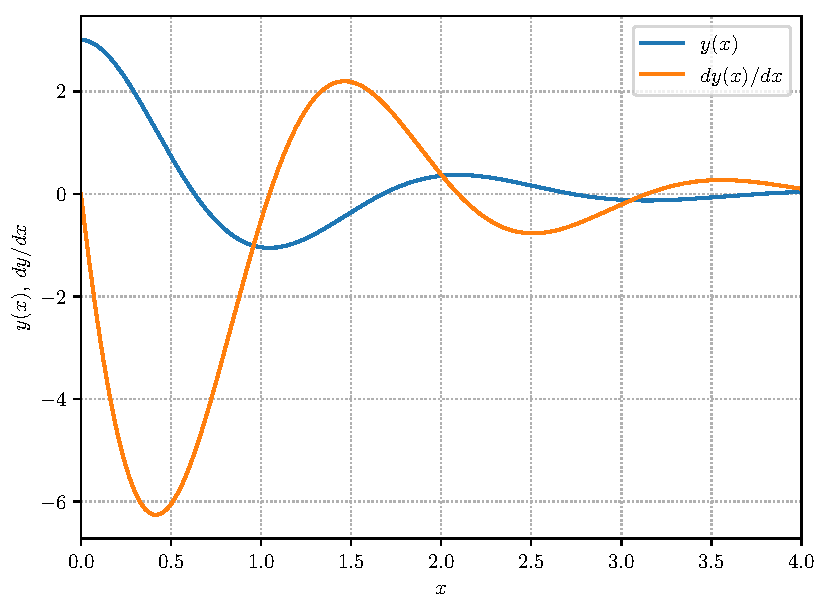
\includegraphics[width=0.75\textwidth]{mixed-fig.pdf}}{Failed to create pdf plot.}
   \captionof{figure}{The function and its derivative.}
\end{minipage}

\end{document}
   % all Python output from mixed.tex
      \documentclass[12pt]{article}
\usepackage{pylatex}
\usepackage{mpllatex}
\usepackage{geometry}
\usepackage{amsmath}
\usepackage{pgf}
\usepackage{caption}
\usepackage{hyperref}
\usepackage{examples}

% portrait
\geometry{papersize={210mm,297mm},hmargin=2cm,tmargin=1.0cm,bmargin=1.5cm}
\parskip=8pt plus 4pt minus 2pt

% landscape
% \geometry{papersize={297mm,210mm},hmargin=2cm,tmargin=1.0cm,bmargin=1.5cm}
% \parskip=6pt plus 3pt minus 2pt

\begin{document}

\section*{A mixed Maple-Python example}

This example demonstrates a cooperative effort where Maple is used to do the analytic computations while Python is used to plot the data.

The example chosen here is to find and plot the solution to the boundary value problem defined by
\begin{align*}
   \frac{d^2y}{dx^2} + 2 \frac{dy}{dx} +10 y = 0\quad\quad\text{with }y(0)=3,\> y'(0)=0
\end{align*}

This example requires two passes, once for Maple and once for Python (and in that order). This example can be run using

\vspace{5pt}

\begin{lstlisting}
   mpllatex.sh -x -i mixed
   pylatex.sh  -x -i mixed
   pdflatex          mixed
\end{lstlisting}

\vspace{5pt}

Note that the last pair of commands could also be combined as {\small\tt pylatex.sh -i mixed}.

\subsection*{The Maple code}

Here Maple is used to first find the general solution of th differential equation. The boundary conitions are then imposed and finally a uniform sampling of the solution is written to a file for later use by Python and Matplotlib.

\begin{maple}
   # a second order ode
   ode := diff(y(x), x, x) + 2*diff(y(x),x) + 10*y(x) = 0:  # mpl (ans.101,ode)

   # find the general solution
   ans := dsolve(ode):                     # mpl (ans.102,ans)

   # set initial conditions
   ics := y(0) = 3, (D(y))(0) = 0:
   tmp := {ics}:                           # mpl (ans.103,tmp)

   # find the particular solution
    f := rhs(dsolve([ics, ode])):          # mpl (ans.104,f)
   df := diff(f,x):                        # mpl (ans.105,df)

    y := x -> f:
   dy := x -> df:

   # now sample y and dy at selected points
   a,b,n := 0.0,2.0*Pi,300:        # domain and number of samples
   dx := (b-a)/n:                  # uniform step

   fd := fopen ("mixed.txt", WRITE):
   for i from 0 to n by 1 do
      x := a + dx*i:
      fprintf(fd,"% .10e % .10e % .10e\n",x,evalf(y(x)),evalf(dy(x))):
   end do:
   fclose(fd):
\end{maple}

The general solution of the differential equation is
\begin{equation*}
  \mpl{ans.102}
\end{equation*}
while the particular solution satifying the boundary conditions is given by
\vspace{5pt}
\begin{align*}
    y(x) &= \mpl{ans.104}
\end{align*}

\subsection*{The Python code}

This is a straighforward use of Matplotlib to plot two functions. The code reads the datafile created previously by Maple and then calls Matplotlib to plot that data.

\begin{python}
   import numpy as np
   import matplotlib.pyplot as plt

   plt.matplotlib.rc('text', usetex = True)
   plt.matplotlib.rc('grid', linestyle = 'dotted')
   plt.matplotlib.rc('figure', figsize = (5.5,4.1)) # (width,height) inches

   x, y, dy = np.loadtxt ('mixed.txt', unpack=True)

   plt.plot (x,y)
   plt.plot (x,dy)

   plt.xlim (0.0,4.0)

   plt.legend(('$y(x)$', '$dy(x)/dx$'), loc = 0)
   plt.xlabel('$x$')
   plt.ylabel('$y(x),\> dy/dx$')
   plt.grid(True)
   plt.tight_layout(0.5)

   plt.savefig('mixed-fig.pdf')
\end{python}

\vspace{10pt}

\begin{minipage}{\textwidth}
   \centering
   \IfFileExists{mixed-fig.pdf}%
   {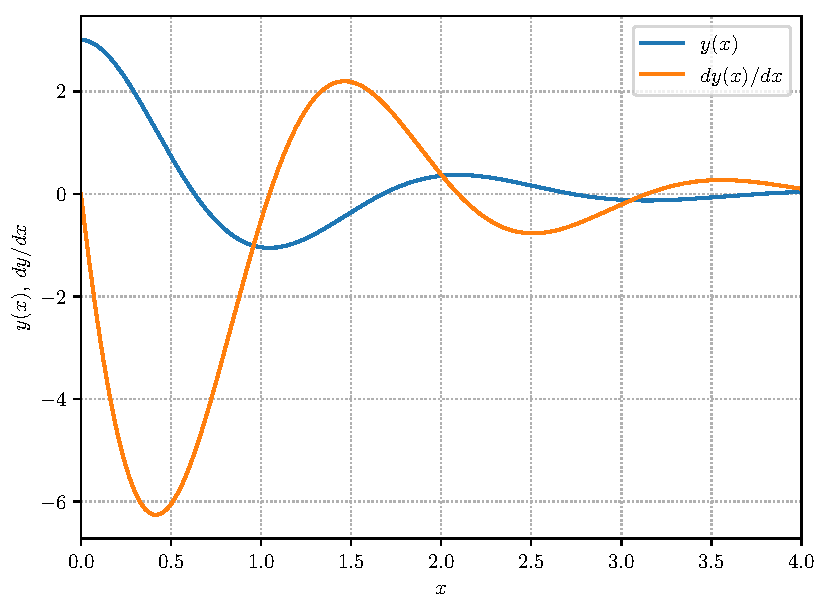
\includegraphics[width=0.75\textwidth]{mixed-fig.pdf}}{Failed to create pdf plot.}
   \captionof{figure}{The function and its derivative.}
\end{minipage}

\end{document}
  % all Maple output from mixed.tex
      ...
      \begin{gather*}
        \mpl{ans.102}       % the Maple output
        \py{ans.102}        % the Python output
      \end{gather*}
      ...
   \end{document}
\end{latex}
\end{minipage}

\vspace{10pt}

Note that care must be taken to avoid name clashes across tags from different sources. If two or more sources define tags with the same name (e.g., {\tt\small foo.pytex} and {\tt\small bah.pytex} both define {\tt\small\verb|\pytag{ans.101}|}) then the last definition will be used. This problem does not arise when the shared tag name, e.g., {\tt\small rhs.101}, occurs in two different languages, such as one in Python and the other in Maple. This can be seen below where the first and last examples both refer to the name {\tt\small ans.102}.

\vspace{10pt}

Note also that the lines

\vspace{5pt}

\begin{latex}
   \usepackage{pylatex}    % so that we can use \py{foo}
   \usepackage{mpllatex}   % so that we can use \mpl{bah}
\end{latex}

\vspace{5pt}

are not essential -- they can be left out but only if the {\tt\small -I} option was supplied when compiling the source. For example, if the {\tt\small pylatex.sty} and {\tt\small mpllatex.sty} files were located in {\tt\small /users/foo/tex/} then the file {\tt\small bah.tex} (containing both Python and Maple code) could be compiled using

\vspace{5pt}

\begin{lstlisting}
   pylatex.sh  -xi bah -I/users/foo/tex/pylatex.sty
   mpllatex.sh -xi bah -I/users/foo/tex/mpllatex.sty
\end{lstlisting}

\vspace{10pt}

This will produce {\tt\small bah.pytex} and {\tt\small bah.mpltex} each containing not only the selected output from {\tt\small bah.tex} but also the definitions of the \pyLaTeX\ and \mplLaTeX\ macros. The {\tt\small -x} option excludes processing of the output by LaTeX.

\section*{Example 1}

\documentclass[12pt]{mpllatex}
\usepackage{examples}

\begin{document}

\section*{Elementary maths}

\begin{maple}
   ans := expand((a+b)^3):                                  # mpl (ans.101,ans)
   ans := factor(-2*x+2*x+a*x-x^2+a*x^2-x^3):               # mpl (ans.102,ans)
   ans := {solve(x^2-4 = 0,x)}:                             # mpl (ans.103,ans) {...} avoids maple/latex syntax error
   sol := solve(x^2-4 = 0,x):                               # multiple roots, can't use mpl(foo,bah) here
   ans := {x=sol[1],x=sol[2]}:                              # mpl (ans.104,ans) fixes problem of multiple roots
   ans := solve({2*a-b = 3, a+b+c = 1,-b+c = 6},{a,b,c}):   # mpl (ans.105,ans)
   ans := evalf[50](Pi):                                    # mpl (ans.106,ans)
   ans := convert(1/((1 + x)*(5 + x)),parfrac):             # mpl (ans.107,ans)
   ans := simplify((1/(1 + x) - 1/(5 + x))/4):              # mpl (ans.108,ans)
   ans := simplify(tanh(ln(x))):                            # mpl (ans.109,ans)
   ans := simplify(tanh(I*x)):                              # mpl (ans.110,ans)
   ans := simplify(sinh(3*x) - 3*sinh(x) - 4*(sinh(x))^3):  # mpl (ans.111,ans)
   ans := ''tanh(ln(x))'':                                  # mpl (lhs.109,ans)
   ans := ''tanh(I*x)'':                                    # mpl (lhs.110,ans)
   ans := ''sinh(3*x) - 3*sinh(x) - 4*(sinh(x))^3'':        # mpl (lhs.111,ans)
\end{maple}

\begin{minipage}[t]{0.65\textwidth}
\begin{align*}
   &\mpl*{ans.101}\\
   &\mpl*{ans.102}\\
   &\mpl*{ans.103}\\
   &\mpl*{ans.104}\\
   &\mpl*{ans.105}\\
   &\mpl*{ans.106}\\
   &\mpl*{ans.107}\\
   &\mpl*{ans.108}\\
   \mpl{lhs.109} &= \Mpl{ans.109}\\
   \mpl{lhs.110} &= \Mpl{ans.110}\\
   \mpl{ans.111} &= \Mpl{lhs.111}
\end{align*}
\end{minipage}
\hskip 1cm
\lower16pt\hbox{%
\begin{minipage}[t]{0.35\textwidth}
\begin{latex}
   \begin{align*}
      &\mpl*{ans.101}\\
      &\mpl*{ans.102}\\
      &\mpl*{ans.103}\\
      &\mpl*{ans.104}\\
      &\mpl*{ans.105}\\
      &\mpl*{ans.106}\\
      &\mpl*{ans.107}\\
      &\mpl*{ans.108}\\
      \mpl{lhs.109} &= \Mpl{ans.109}\\
      \mpl{lhs.110} &= \Mpl{ans.110}\\
      \mpl{ans.111} &= \Mpl{lhs.111}
   \end{align*}
\end{latex}
\end{minipage}}

\clearpage

\section*{Linear Algebra}

\begin{minipage}[t]{0.65\textwidth}
\begin{maple}
   with(LinearAlgebra):
   mat  := <<2|3>, <5|4>>:                        # mpl (ans.201,mat)
   ans  := Eigenvectors(mat,output='list'):
   eig1 := ans[1][1]:                             # 1st eigenvalue
   eig2 := ans[2][1]:                             # 2nd eigenvalue
   v1   := ans[1][3][1]:                          # 1st eigenvector
   v2   := ans[2][3][1]:                          # 2nd eigenvector
   eig  := <eig1,eig2>:                           # mpl (ans.202,eig)
   ans  := <v1|v2>:                               # mpl (ans.203,ans)
   ans  := CharacteristicPolynomial(mat,lambda):  # mpl (ans.204,ans)
   vec  := <3,7>:                                 # mpl (ans.205,vec)
   sol  := LinearSolve(mat,vec):                  # mpl (ans.206,sol)
\end{maple}
\end{minipage}
\hskip 1cm
\begin{minipage}[t]{0.35\textwidth}
\begin{latex}
   \begin{align*}
      &\mpl*{ans.201}\\
      &\mpl*{ans.202}\\
      &\mpl*{ans.203}\\
      &\mpl*{ans.204}\\
      &\mpl*{ans.205}\\
      &\mpl*{ans.206}
   \end{align*}
\end{latex}
\end{minipage}

\begin{align*}
   &\mpl*{ans.201}\\
   &\mpl*{ans.202}\\
   &\mpl*{ans.203}\\
   &\mpl*{ans.204}\\
   &\mpl*{ans.205}\\
   &\mpl*{ans.206}
\end{align*}

\clearpage

\section*{Limits}

\begin{minipage}[t]{0.65\textwidth}
\begin{maple}
   ans := limit(sin(4*x)/x,x=0):                  # mpl (ans.301,ans)
   ans := limit(2^x/x,x=infinity):                # mpl (ans.302,ans)
   ans := limit(((x+dx)^2 - x^2)/dx, dx=0):       # mpl (ans.303,ans)
   ans := limit((4*n + 1)/(3*n - 1),n=infinity):  # mpl (ans.304,ans)
   ans := limit((1+(a/n))^n,n=infinity):          # mpl (ans.305,ans)
\end{maple}
\end{minipage}
\hskip 1cm
\begin{minipage}[t]{0.35\textwidth}
\begin{latex}
   \begin{align*}
      &\mpl*{ans.301}\\
      &\mpl*{ans.302}\\
      &\mpl*{ans.303}\\
      &\mpl*{ans.304}\\
      &\mpl*{ans.305}
   \end{align*}
\end{latex}
\end{minipage}

\vspace{-10pt}

\begin{align*}
   &\mpl*{ans.301}\\
   &\mpl*{ans.302}\\
   &\mpl*{ans.303}\\
   &\mpl*{ans.304}\\
   &\mpl*{ans.305}
\end{align*}

\section*{Series}

\begin{minipage}[t]{0.65\textwidth}
\begin{maple}
   ans := series((1 + x)^(-2), x=1, 6):          # mpl (ans.401,ans)
   ans := series(exp(x), x=0, 6):                # mpl (ans.402,ans)
   ans := sum(1/n^2, n=1..50):                   # mpl (ans.403,ans)
   ans := sum(1/n^4, n=1..infinity):             # mpl (ans.404,ans)
\end{maple}
\end{minipage}
\hskip 1cm
\begin{minipage}[t]{0.35\textwidth}
\begin{latex}
   \begin{align*}
      &\mpl*{ans.401}\\
      &\mpl*{ans.402}\\
      &\mpl*{ans.403}\\
      &\mpl*{ans.404}
   \end{align*}
\end{latex}
\end{minipage}

\begin{align*}
   &\mpl*{ans.401}\\
   &\mpl*{ans.402}\\
   &\mpl*{ans.403}\\
   &\mpl*{ans.404}
\end{align*}

\clearpage

\section*{Calculus}

\begin{minipage}[t]{0.65\textwidth}
\begin{maple}
   ans := diff(x*sin(x),x):                          # mpl (ans.501,ans)
   ans := eval(diff(x*sin(x),x),x=Pi/4):             # mpl (ans.502,ans)
   ans := int(2*sin(x)^2, x=a..b):                   # mpl (ans.503,ans)
   ans := int(2*exp(-x^2),x=0..infinity):            # mpl (ans.504,ans)
   ans := ''int(2*exp(-x^2),x=0..infinity)'':        # mpl (lhs.504,ans)
   ans := int(int(x^2 + y^2,  y=0..x),x=0..1):       # mpl (ans.505,ans)
   ans := ''int(int(x^2 + y^2,  y=0..x),x=0..1)'':   # mpl (lhs.505,ans)
\end{maple}
\end{minipage}
\hskip 1cm
\begin{minipage}[t]{0.35\textwidth}
\begin{latex}
   \begin{align*}
      &\mpl*{ans.501}\\
      &\mpl*{ans.502}\\
      &\mpl*{ans.503}\\
      \mpl{lhs.504}&=\Mpl{ans.504}\\
      \mpl{lhs.505}&=\Mpl{ans.505}
   \end{align*}
\end{latex}
\end{minipage}

\begin{align*}
   &\mpl*{ans.501}\\
   &\mpl*{ans.502}\\
   &\mpl*{ans.503}\\
   \mpl{lhs.504}&=\Mpl{ans.504}\\
   \mpl{lhs.505}&=\Mpl{ans.505}
\end{align*}

\clearpage

\section*{Differential equations}

\begin{minipage}[t]{0.65\textwidth}
\begin{maple}
   ode := diff(y(x),x) + y(x) = 2*a*sin(x):
   ics := y(0) = 0:
   ans := rhs(dsolve(ode)):                    # mpl (ans.601,ans)
   ans := rhs(dsolve([ics,ode])):              # mpl (ans.602,ans)

   ode := diff(y(x),x,x) + y(x) = 0:
   ics := y(0)=0, (D(y))(0) = 1:
   ans := rhs(dsolve(ode)):                    # mpl (ans.603,ans)
   ans := rhs(dsolve([ics,ode])):              # mpl (ans.604,ans)

   ode := diff(y(x),x,x) + 5*diff(y(x),x) - 6*y(x) = 0:
   ans := rhs(dsolve(ode)):                    # mpl (ans.605,ans)
   sol := eval(ans,[_C1=2,_C2=3]):             # mpl (ans.606,sol)
\end{maple}
\end{minipage}
\hskip 1cm
\begin{minipage}[t]{0.35\textwidth}
\begin{latex}
   \begin{align*}
      &\mpl*{ans.601}\\
      &\mpl*{ans.602}\\
      &\mpl*{ans.603}\\
      &\mpl*{ans.604}\\
      &\mpl*{ans.605}\\
      &\mpl*{ans.606}
   \end{align*}
\end{latex}
\end{minipage}

\begin{align*}
   &\mpl*{ans.601}\\
   &\mpl*{ans.602}\\
   &\mpl*{ans.603}\\
   &\mpl*{ans.604}\\
   &\mpl*{ans.605}\\
   &\mpl*{ans.606}
\end{align*}

\end{document}


\begin{align*}
   &\py*{ans.102}\\
   &\py*{ans.302}\\
   &\py*{ans.303}\\
   &\py*{ans.305}\\
   &\py*{ans.401}\\
   &\py*{ans.402}\\
   &\py*{ans.403}\\
   &\py*{ans.404}
\end{align*}

\section*{Example 2}

% based on example 7 in pythontex_gallery
% https://github.com/gpoore/pythontex/

\documentclass[12pt]{mpllatex}
\usepackage{examples}

\begin{document}

\section*{A table of derivatives and anti-derivatives}

This example is based upon a nice example in the Pythontex gallery, see
\ \url{https://github.com/gpoore/pythontex/}.
It uses a tagged block to capture the Maple output for later use
in the body of the LaTeX table.

\lstset{numbers=left}

\begin{minipage}[t]{0.75\textwidth}
\begin{maple}
   # Create a list of functions to include in the table
   funcs := [[sin(x),"\\\\"],         [cos(x),"\\\\"],         [tan(x),"\\\\"],
             [arcsin(x),"\\\\[5pt]"], [arccos(x),"\\\\[5pt]"], [arctan(x),"\\\\[5pt]"],
             [sinh(x),"\\\\"],        [cosh(x),"\\\\"],        [tanh(x)," "]]:

   # mplBeg (CalculusTable)
   for foo in funcs do
       func := foo[1]:
       eol  := foo[2]:
       myddx := ''diff''(func,x):
       myint := ''int''(func,x):
       Print(cat(Latex(myddx),"&=",Latex(diff(func,x)),"\\quad & \\quad")):
       Print(cat(Latex(myint),"&=",Latex(int(func,x)),eol)):
   end do:
   # mplEnd (CalculusTable)
\end{maple}
\end{minipage}
\hskip 1cm
\begin{minipage}[t]{0.25\textwidth}
\begin{latex}
   \begin{align*}
      \mpl {CalculusTable}
   \end{align*}
\end{latex}
\end{minipage}

\clearpage

\begin{align*}
   \mpl {CalculusTable}
\end{align*}

\end{document}


\begin{align*}
   \py {CalculusTable}
\end{align*}

\section*{Example 3}

\documentclass[12pt]{cdblatex}
\usepackage{examples}

\begin{document}

\section*{Curvature of a 2-sphere}

This examples uses standard methods to compute the scalar curvature of a 2-sphere.

\begin{cadabra}
   {\theta, \varphi}::Coordinate.
   {\alpha, \beta, \gamma, \delta, \rho, \sigma, \mu, \nu, \lambda}::Indices(values={\varphi, \theta}, position=independent).

   \partial{#}::PartialDerivative.

   g_{\alpha\beta}::Metric.
   g^{\alpha\beta}::InverseMetric.

   Chr := \Gamma^{\alpha}_{\mu\nu} -> 1/2 g^{\alpha\beta} (  \partial_{\nu}{g_{\beta\mu}}
                                                           + \partial_{\mu}{g_{\beta\nu}}
                                                           - \partial_{\beta}{g_{\mu\nu}} ).

   Rabcd := R^{\rho}_{\sigma\mu\nu} ->   \partial_{\mu}{\Gamma^{\rho}_{\sigma\nu}}
                                       - \partial_{\nu}{\Gamma^{\rho}_{\sigma\mu}}
                                       + \Gamma^{\rho}_{\beta\mu} \Gamma^{\beta}_{\sigma\nu}
                                       - \Gamma^{\rho}_{\beta\nu} \Gamma^{\beta}_{\sigma\mu}.

   Rab := R_{\sigma\nu} -> R^{\rho}_{\sigma\rho\nu}.

   R := R -> R_{\sigma\nu} g^{\sigma\nu}.

   gab:={ g_{\theta\theta}   = r**2,
          g_{\varphi\varphi} = r**2 \sin(\theta)**2 }.   # cdb(gab,gab)

   complete   (gab, $g^{\alpha\beta}$)                   # cdb(iab,gab)

   evaluate   (Chr, gab, rhsonly=True)                   # cdb(Chr,Chr)

   substitute (Rabcd, Chr)
   evaluate   (Rabcd, gab, rhsonly=True)                 # cdb(Rabcd,Rabcd)

   substitute (Rab, Rabcd)
   evaluate   (Rab, gab, rhsonly=True)                   # cdb(Rab,Rab)

   substitute (R, Rab)
   evaluate   (R, gab, rhsonly=True)                     # cdb(R,R)
\end{cadabra}

\begin{minipage}[t]{0.65\textwidth}
\begin{align*}
   &\cdb{iab}\\[10pt]
   &\cdb{Chr}\\[10pt]
   &\cdb{Rabcd}\\[10pt]
   &\cdb{Rab}\\[10pt]
   &\cdb{R}
\end{align*}
\end{minipage}
\hskip 1cm
\lower16pt\hbox{%
\begin{minipage}[t]{0.35\textwidth}
\begin{latex}
   \begin{align*}
      &\cdb{iab}\\[10pt]
      &\cdb{Chr}\\[10pt]
      &\cdb{Rabcd}\\[10pt]
      &\cdb{Rab}\\[10pt]
      &\cdb{R}
   \end{align*}
\end{latex}
\end{minipage}}

\end{document}


\begin{align*}
   \py{lhs.01} &= \py{rhs.01}\\
               &= \py{rhs.02}\\
               &= \py{rhs.03}\\
               &= \py{rhs.04}\\
               &\approx \py{rhs.05}
\end{align*}

\clearpage

\section*{Example 4}

\begin{minipage}{\textwidth}
   \centering
   \IfFileExists{example-04-fig.pdf}%
   % {\scalebox{0.75}{\input{example-04-fig.pdf}}}{Failed to create plot.}
   {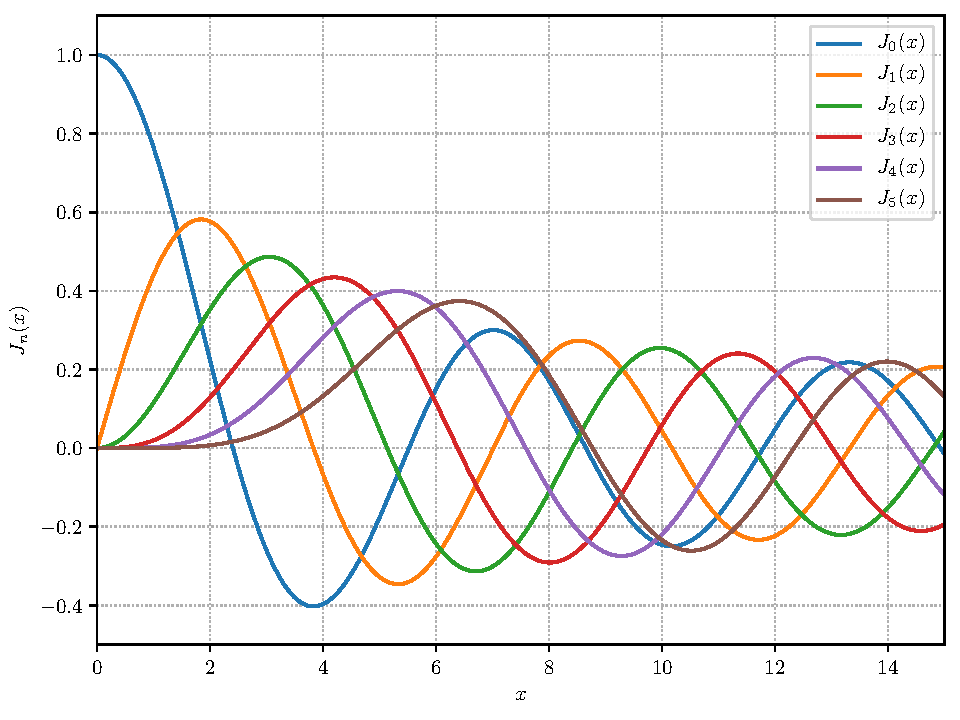
\includegraphics[width=6.4in]{example-04-fig.pdf}}{Failed to create plot.}
   \captionof{figure}{The first six Bessel functions.}
\end{minipage}

\section*{Example 5}

\documentclass[12pt]{pylatex}
\usepackage{examples}

\begin{document}

\section*{Displaying long expressions}

This example uses a simple (though contrived) example of a Taylor series expansion of $1/(1+x)$ to demonstrate the problems that can arise when displaying very long expressions.

% \vspace{12pt}

\begin{minipage}[t]{0.50\textwidth}
\begin{python}
   from sympy import *
   x = Symbol('x')
   ans    = 1/(1+x)                 # py (ans.511,ans)
   taylor = ans.series(x, 0, 10)    # py (ans.512,taylor)
   taylor = ans.series(x, 0, 20)    # py (ans.513,taylor)
   taylor = ans.series(x, 0, 23)    # py (ans.514,taylor)
\end{python}
\end{minipage}
\hskip 0.5cm
\begin{minipage}[t]{0.50\textwidth}
\begin{latex}
   \begin{dgroup*}[spread={5pt}]
      \begin{dmath*} f(x) = \Py*{ans.511} \end{dmath*}
      \begin{dmath*}    {}= \Py*{ans.512} \end{dmath*}
      \begin{dmath*}    {}= \Py*{ans.513} \end{dmath*}
      \begin{dmath*}    {}= \Py*{ans.514} \end{dmath*}
      \begin{dmath*}    {}= \Py*[\hskip 2cm]{ans.514} \end{dmath*}
   \end{dgroup*}
\end{latex}
\end{minipage}

\vspace{18pt}

The first four lines of the following output were set using {\tt\small\verb|\Py*|}
while the final line used {\tt\small\verb|\Py*[\hskip=2cm]|}. The last pair of lines displays
the output for the same tag {\tt\small ans.514} and clearly the formatting of the second
last line is not ideal as the text has overlapped the tag. This was corrected in the final
line by using the optional argument {\tt\small\verb|[\hskip=2cm]|} in the call to {\tt\small\verb|\Py*|}.

\begin{dgroup*}[spread={5pt}]
   \begin{dmath*} f(x) = \Py*{ans.511} \end{dmath*}
   \begin{dmath*}    {}= \Py*{ans.512} \end{dmath*}
   \begin{dmath*}    {}= \Py*{ans.513} \end{dmath*}
   \begin{dmath*}    {}= \Py*{ans.514} \end{dmath*}
   \begin{dmath*}    {}= \Py*[\hskip 2cm]{ans.514} \end{dmath*}
\end{dgroup*}

\end{document}


\begin{dgroup*}[spread={5pt}]
   \begin{dmath*} f(x) = \Py*{ans.511} \end{dmath*}
   \begin{dmath*}    {}= \Py*{ans.512} \end{dmath*}
   \begin{dmath*}    {}= \Py*{ans.513} \end{dmath*}
   \begin{dmath*}    {}= \Py*{ans.514} \end{dmath*}
   \begin{dmath*}    {}= \Py*{ans.514} \end{dmath*}% LCB: do we need extar space for the tag?
\end{dgroup*}

\section*{Example 6}

\documentclass[12pt]{cdblatex}
\usepackage{examples}

\begin{document}

\section*{The Gauss relation for the curvature of a hypersurface}

\begin{cadabra}
   {a,b,c,d,e,f,g,i,j,k,l,m,n,o,p,q,r,s,t,u#}::Indices.

   \nabla_{#}::Derivative.

   K_{a b}::Symmetric.
   g^{a}_{b}::KroneckerDelta.

   # Define the projection operator

   hab:=h^{a}_{b} -> g^{a}_{b} - n^{a} n_{b}.

   # 3-covariant derivative obtained by projection on 4-covariant derivative

   vpq:=v_{p q} -> h^{a}_{p} h^{b}_{q} \nabla_{b}{v_{a}}.

   # Compute 3-curvature by commutation of covariant derivatives

   vpqr:= h^{a}_{p} h^{b}_{q} h^{c}_{r} ( \nabla_{c}{v_{a b}} - \nabla_{b}{v_{a c}} ).

   substitute (vpq,hab)
   substitute (vpqr,vpq)

   distribute   (vpqr)
   product_rule (vpqr)
   distribute   (vpqr)
   eliminate_kronecker(vpqr)

   # Standard substitutions

   substitute (vpqr,$h^{a}_{b} n^{b} -> 0$)
   substitute (vpqr,$h^{a}_{b} n_{a} -> 0$)
   substitute (vpqr,$\nabla_{a}{g^{b}_{c}} -> 0$)
   substitute (vpqr,$n^{a} \nabla_{b}{v_{a}} -> -v_{a} \nabla_{b}{n^{a}}$)
   substitute (vpqr,$v_{a} \nabla_{b}{n^{a}} -> v_{p} h^{p}_{a}\nabla_{b}{n^{a}}$)
   substitute (vpqr,$h^{p}_{a} h^{q}_{b} \nabla_{p}{n_{q}} -> K_{a b}$)
   substitute (vpqr,$h^{p}_{a} h^{q}_{b} \nabla_{p}{n^{b}} -> K_{a}^{q}$)

   # Tidy up and display the results

   {h^{a}_{b},\nabla_{a}{v_{b}}}::SortOrder.

   sort_product   (vpqr)
   rename_dummies (vpqr)
   canonicalise   (vpqr)
   factor_out     (vpqr,$h^{a?}_{b?}$)
   factor_out     (vpqr,$v_{a?}$)       # cdb(gauss,vpqr)
\end{cadabra}

\subsection*{The Gauss relation for the curvature of a hypersurface}

\begin{align*}
   D_{r}(D_{q}v_p) - D_{q}(D_{r}v_p) = \cdb{gauss}
\end{align*}

\vspace{15pt}

\begin{latex}
   \begin{align*}
      D_{r}(D_{q}v_p) - D_{q}(D_{r}v_p) = \cdb{gauss}
   \end{align*}
\end{latex}

\end{document}


\def\eps{\epsilon}
\def\RuleA{\vrule depth0pt  width0pt height14pt}
\def\RuleB{\vrule depth8pt  width0pt height14pt}
\def\RuleC{\vrule depth10pt width0pt height16pt}

\setlength{\tabcolsep}{0.025\textwidth}%

\vspace{20pt}

\begin{center}
\begin{tabular}{cccc}%
   \noalign{\hrule height 1pt}
   \multicolumn{4}{c}{\RuleC\rmfamily\bfseries%
   Newton-Raphson iterations \quad%
   $x_{n+1} = x_n - f_n/f'_n\ ,\quad f(x) = x-e^{-x}$}\\
   \noalign{\hrule height 1pt}
   \RuleB$ n$&$ x_n$&$ \eps_{n} =  x_{n} - e^{-x_{n}}$&$\eps_{n}/\eps_{n-1}^2$\\
   \noalign{\hrule height 0.5pt}
   \py{table}
   \noalign{\hrule height 1pt}
\end{tabular}
\end{center}

\section*{Example 7}

\documentclass[12pt]{cdblatex}
\usepackage{examples}

\lstset{numbers=left}

\begin{document}

\section*{The metric connection in Riemann normal coordinates}

In local Riemann normal coordinates, the metric components can always be expanded as a power series in the Riemann curvatures and its derivatives (provided the curvatives are finite at the expansion point). In particular
\begin{align*}
   g_{ab}(x) &= g_{a b} - \frac{1}{3} x^{c} x^{d} R_{a c b d}
                        - \frac{1}{6} x^{c} x^{d} x^{e} \nabla_{c}{R_{a d b e}} + \cdots\\
   g^{ab}(x) &= g^{a b} + \frac{1}{3} x^{c} x^{d} g^{a e} g^{b f} R_{c e d f}
                        + \frac{1}{6} x^{c} x^{d} x^{e} g^{a f} g^{b g} \nabla_{c}{R_{d f e g}} + \cdots
\end{align*}
where $g_{ab}$ and $g^{ab}$ are independent of the coordinates $x^a$ and where $\nabla$ is the metric compatable derivative operator (i.e., $\nabla(g)=0$). In applications in General Relativity the $g_{ab}$ are often chosen to be $g_{ab} = {\rm diag}(-1,1,1,1)$.

Here we will use the standard metric compatible connection
\begin{align*}
   \Gamma^{d}_{ab}(x) = \frac{1}{2} g^{dc}\left( g_{cb,a} + g_{ac,b} - g_{ab,c} \right)
\end{align*}
to compute $\Gamma^{d}_{ab}(x)$ to terms linear in $R_{abcd}$ and $\nabla_{e} R_{abcd}$.

\vspace{12pt}

\begin{cadabra}
   {a,b,c,d,e,f,g,h,i,j,k,l,m,n,o,p,q,r,s,t,u,v,w#}::Indices(position=independent).

   D{#}::PartialDerivative.
   \nabla{#}::Derivative.

   g_{a b}::Metric.
   g^{a b}::InverseMetric.

   \delta{#}::KroneckerDelta.

   R_{a b c d}::RiemannTensor.

   x^{a}::Depends(D{#}).
   x^{a}::Weight(label=num,value=1).

   R_{a b c d}::Depends(\nabla{#}).

   DxaDxb := D_{a}{x^{b}}->\delta^{b}_{a}.

   # can chose lower order approximations by truncating the following pair

   gab := g_{a b} - 1/3 x^{c} x^{d} R_{a c b d}
                  - 1/6 x^{c} x^{d} x^{e} \nabla_{c}{R_{a d b e}}.                    # cdb(gab.000,gab)

   iab := g^{a b} + 1/3 x^{c} x^{d} g^{a e} g^{b f} R_{c e d f}
                  + 1/6 x^{c} x^{d} x^{e} g^{a f} g^{b g} \nabla_{c}{R_{d f e g}}.    # cdb(iab.000,iab)

   gab := g_{a b} -> @(gab).
   iab := g^{a b} -> @(iab).

   gam := 1/2 g^{d c} (D_{a}{g_{c b}} + D_{b}{g_{a c}} - D_{c}{g_{a b}}).             # cdb(gam.001,gam)

   substitute   (gam,gab)
   substitute   (gam,iab)
   distribute   (gam)              # cdb(gam.002,gam)
   unwrap       (gam)              # cdb(gam.003,gam)
   product_rule (gam)              # cdb(gam.004,gam)
   distribute   (gam)              # cdb(gam.005,gam)
   substitute   (gam,DxaDxb)       # cdb(gam.006,gam)
   eliminate_kronecker (gam)       # cdb(gam.007,gam)
   sort_product   (gam)            # cdb(gam.008,gam)
   rename_dummies (gam)            # cdb(gam.009,gam)
   canonicalise   (gam)            # cdb(gam.010,gam)

   def truncate (obj,n):

       ans = Ex(0)  # create a Cadabra object with value zero

       for i in range (0,n+1):
          foo := @(obj).
          bah  = Ex("num = " + str(i))
          distribute  (foo)
          keep_weight (foo, bah)
          ans = ans + foo

       return ans

   gam = truncate (gam,2)   # cdb (gam.101,gam)  # allow up to 2nd order in x^a

   # ==========================================================================
   # the remaining code is just for pretty printing

   {x^{a},g^{a b},R_{a b c d},\nabla_{e}{R_{a b c d}}}::SortOrder.

   def get_term (obj,n):

       foo := @(obj).
       bah  = Ex("num = " + str(n))
       distribute  (foo)
       keep_weight (foo, bah)

       return foo

   def reformat (obj,scale):

      foo  = Ex(str(scale))
      bah := @(foo) @(obj).

      distribute     (bah)
      sort_product   (bah)
      rename_dummies (bah)
      canonicalise   (bah)
      factor_out     (bah,$x^{a?},g^{b? c?}$)
      ans := @(bah) / @(foo).

      return ans

   gam1 = get_term (gam,1)       # cdb (gam1.301,gam1)
   gam2 = get_term (gam,2)       # cdb (gam2.301,gam2)

   gam1 = reformat (gam1,  3)    # cdb (gam1.301,gam1)
   gam2 = reformat (gam2, 12)    # cdb (gam2.301,gam2)

   Gamma  := @(gam1) + @(gam2).  # cdb (Gamma.301,Gamma)
   Scaled := 12 @(Gamma).        # cdb (Scaled.301,Scaled)

\end{cadabra}

\subsection*{The metric connection in Riemann normal coordinates}

\begin{dgroup*}
   \begin{dmath*} \Gamma^{d}_{a b} = \cdb{Gamma.301} \end{dmath*}
\end{dgroup*}

\begin{dgroup*}
   \begin{dmath*} 12 \Gamma^{d}_{a b} = \cdb{Scaled.301} \end{dmath*}
\end{dgroup*}

\vspace{20pt}

\begin{latex}
   \begin{dgroup*}
      \begin{dmath*} \Gamma^{d}_{a b} = \cdb{Gamma.301} \end{dmath*}
   \end{dgroup*}

   \begin{dgroup*}
      \begin{dmath*} 12 \Gamma^{d}_{a b} = \cdb{Scaled.301} \end{dmath*}
   \end{dgroup*}
\end{latex}

% uncomment the following to get more detail of the computations

% \begin{dgroup*}
%    \begin{dmath*} \cdb{gam.002} \end{dmath*}
%    \begin{dmath*} \cdb{gam.003} \end{dmath*}
%    \begin{dmath*} \cdb{gam.004} \end{dmath*}
%    \begin{dmath*} \cdb{gam.005} \end{dmath*}
%    \begin{dmath*} \cdb{gam.006} \end{dmath*}
%    \begin{dmath*} \cdb{gam.007} \end{dmath*}
%    \begin{dmath*} \cdb{gam.008} \end{dmath*}
%    \begin{dmath*} \cdb{gam.009} \end{dmath*}
%    \begin{dmath*} \cdb{gam.010} \end{dmath*}
% \end{dgroup*}

\end{document}


\bgroup\tt
\begin{tabular}{rl}
   \py{info}
\end{tabular}
\egroup

\clearpage

\section*{Python and Maple}

\documentclass[12pt]{article}
\usepackage{pylatex}
\usepackage{mpllatex}
\usepackage{geometry}
\usepackage{amsmath}
\usepackage{pgf}
\usepackage{caption}
\usepackage{hyperref}
\usepackage{examples}

% portrait
\geometry{papersize={210mm,297mm},hmargin=2cm,tmargin=1.0cm,bmargin=1.5cm}
\parskip=8pt plus 4pt minus 2pt

% landscape
% \geometry{papersize={297mm,210mm},hmargin=2cm,tmargin=1.0cm,bmargin=1.5cm}
% \parskip=6pt plus 3pt minus 2pt

\begin{document}

\section*{A mixed Maple-Python example}

This example demonstrates a cooperative effort where Maple is used to do the analytic computations while Python is used to plot the data.

The example chosen here is to find and plot the solution to the boundary value problem defined by
\begin{align*}
   \frac{d^2y}{dx^2} + 2 \frac{dy}{dx} +10 y = 0\quad\quad\text{with }y(0)=3,\> y'(0)=0
\end{align*}

This example requires two passes, once for Maple and once for Python (and in that order). This example can be run using

\vspace{5pt}

\begin{lstlisting}
   mpllatex.sh -x -i mixed
   pylatex.sh  -x -i mixed
   pdflatex          mixed
\end{lstlisting}

\vspace{5pt}

Note that the last pair of commands could also be combined as {\small\tt pylatex.sh -i mixed}.

\subsection*{The Maple code}

Here Maple is used to first find the general solution of th differential equation. The boundary conitions are then imposed and finally a uniform sampling of the solution is written to a file for later use by Python and Matplotlib.

\begin{maple}
   # a second order ode
   ode := diff(y(x), x, x) + 2*diff(y(x),x) + 10*y(x) = 0:  # mpl (ans.101,ode)

   # find the general solution
   ans := dsolve(ode):                     # mpl (ans.102,ans)

   # set initial conditions
   ics := y(0) = 3, (D(y))(0) = 0:
   tmp := {ics}:                           # mpl (ans.103,tmp)

   # find the particular solution
    f := rhs(dsolve([ics, ode])):          # mpl (ans.104,f)
   df := diff(f,x):                        # mpl (ans.105,df)

    y := x -> f:
   dy := x -> df:

   # now sample y and dy at selected points
   a,b,n := 0.0,2.0*Pi,300:        # domain and number of samples
   dx := (b-a)/n:                  # uniform step

   fd := fopen ("mixed.txt", WRITE):
   for i from 0 to n by 1 do
      x := a + dx*i:
      fprintf(fd,"% .10e % .10e % .10e\n",x,evalf(y(x)),evalf(dy(x))):
   end do:
   fclose(fd):
\end{maple}

The general solution of the differential equation is
\begin{equation*}
  \mpl{ans.102}
\end{equation*}
while the particular solution satifying the boundary conditions is given by
\vspace{5pt}
\begin{align*}
    y(x) &= \mpl{ans.104}
\end{align*}

\subsection*{The Python code}

This is a straighforward use of Matplotlib to plot two functions. The code reads the datafile created previously by Maple and then calls Matplotlib to plot that data.

\begin{python}
   import numpy as np
   import matplotlib.pyplot as plt

   plt.matplotlib.rc('text', usetex = True)
   plt.matplotlib.rc('grid', linestyle = 'dotted')
   plt.matplotlib.rc('figure', figsize = (5.5,4.1)) # (width,height) inches

   x, y, dy = np.loadtxt ('mixed.txt', unpack=True)

   plt.plot (x,y)
   plt.plot (x,dy)

   plt.xlim (0.0,4.0)

   plt.legend(('$y(x)$', '$dy(x)/dx$'), loc = 0)
   plt.xlabel('$x$')
   plt.ylabel('$y(x),\> dy/dx$')
   plt.grid(True)
   plt.tight_layout(0.5)

   plt.savefig('mixed-fig.pdf')
\end{python}

\vspace{10pt}

\begin{minipage}{\textwidth}
   \centering
   \IfFileExists{mixed-fig.pdf}%
   {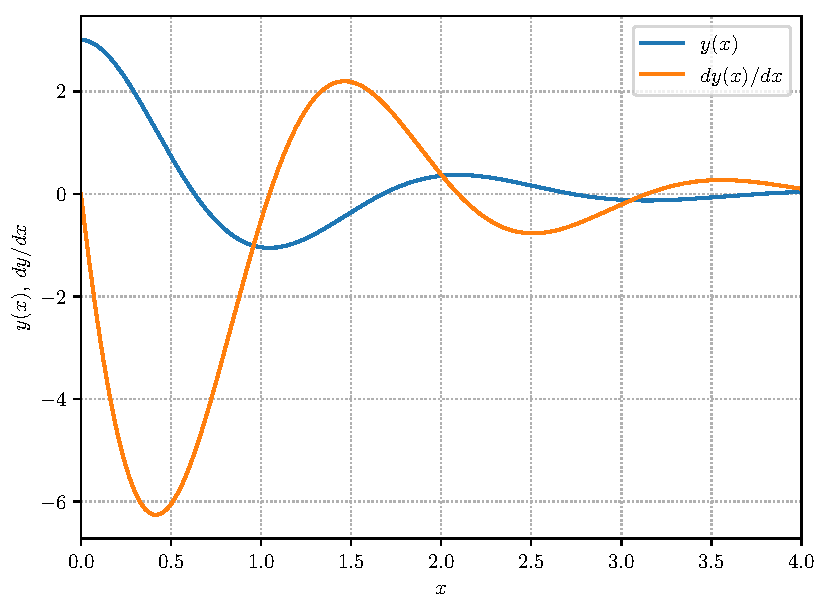
\includegraphics[width=0.75\textwidth]{mixed-fig.pdf}}{Failed to create pdf plot.}
   \captionof{figure}{The function and its derivative.}
\end{minipage}

\end{document}

\documentclass[12pt]{article}
\usepackage{pylatex}
\usepackage{mpllatex}
\usepackage{geometry}
\usepackage{amsmath}
\usepackage{pgf}
\usepackage{caption}
\usepackage{hyperref}
\usepackage{examples}

% portrait
\geometry{papersize={210mm,297mm},hmargin=2cm,tmargin=1.0cm,bmargin=1.5cm}
\parskip=8pt plus 4pt minus 2pt

% landscape
% \geometry{papersize={297mm,210mm},hmargin=2cm,tmargin=1.0cm,bmargin=1.5cm}
% \parskip=6pt plus 3pt minus 2pt

\begin{document}

\section*{A mixed Maple-Python example}

This example demonstrates a cooperative effort where Maple is used to do the analytic computations while Python is used to plot the data.

The example chosen here is to find and plot the solution to the boundary value problem defined by
\begin{align*}
   \frac{d^2y}{dx^2} + 2 \frac{dy}{dx} +10 y = 0\quad\quad\text{with }y(0)=3,\> y'(0)=0
\end{align*}

This example requires two passes, once for Maple and once for Python (and in that order). This example can be run using

\vspace{5pt}

\begin{lstlisting}
   mpllatex.sh -x -i mixed
   pylatex.sh  -x -i mixed
   pdflatex          mixed
\end{lstlisting}

\vspace{5pt}

Note that the last pair of commands could also be combined as {\small\tt pylatex.sh -i mixed}.

\subsection*{The Maple code}

Here Maple is used to first find the general solution of th differential equation. The boundary conitions are then imposed and finally a uniform sampling of the solution is written to a file for later use by Python and Matplotlib.

\begin{maple}
   # a second order ode
   ode := diff(y(x), x, x) + 2*diff(y(x),x) + 10*y(x) = 0:  # mpl (ans.101,ode)

   # find the general solution
   ans := dsolve(ode):                     # mpl (ans.102,ans)

   # set initial conditions
   ics := y(0) = 3, (D(y))(0) = 0:
   tmp := {ics}:                           # mpl (ans.103,tmp)

   # find the particular solution
    f := rhs(dsolve([ics, ode])):          # mpl (ans.104,f)
   df := diff(f,x):                        # mpl (ans.105,df)

    y := x -> f:
   dy := x -> df:

   # now sample y and dy at selected points
   a,b,n := 0.0,2.0*Pi,300:        # domain and number of samples
   dx := (b-a)/n:                  # uniform step

   fd := fopen ("mixed.txt", WRITE):
   for i from 0 to n by 1 do
      x := a + dx*i:
      fprintf(fd,"% .10e % .10e % .10e\n",x,evalf(y(x)),evalf(dy(x))):
   end do:
   fclose(fd):
\end{maple}

The general solution of the differential equation is
\begin{equation*}
  \mpl{ans.102}
\end{equation*}
while the particular solution satifying the boundary conditions is given by
\vspace{5pt}
\begin{align*}
    y(x) &= \mpl{ans.104}
\end{align*}

\subsection*{The Python code}

This is a straighforward use of Matplotlib to plot two functions. The code reads the datafile created previously by Maple and then calls Matplotlib to plot that data.

\begin{python}
   import numpy as np
   import matplotlib.pyplot as plt

   plt.matplotlib.rc('text', usetex = True)
   plt.matplotlib.rc('grid', linestyle = 'dotted')
   plt.matplotlib.rc('figure', figsize = (5.5,4.1)) # (width,height) inches

   x, y, dy = np.loadtxt ('mixed.txt', unpack=True)

   plt.plot (x,y)
   plt.plot (x,dy)

   plt.xlim (0.0,4.0)

   plt.legend(('$y(x)$', '$dy(x)/dx$'), loc = 0)
   plt.xlabel('$x$')
   plt.ylabel('$y(x),\> dy/dx$')
   plt.grid(True)
   plt.tight_layout(0.5)

   plt.savefig('mixed-fig.pdf')
\end{python}

\vspace{10pt}

\begin{minipage}{\textwidth}
   \centering
   \IfFileExists{mixed-fig.pdf}%
   {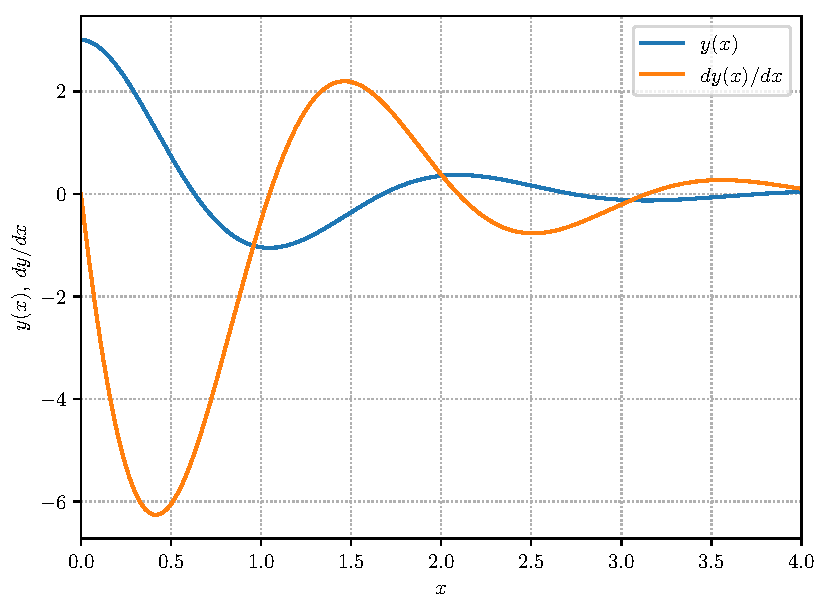
\includegraphics[width=0.75\textwidth]{mixed-fig.pdf}}{Failed to create pdf plot.}
   \captionof{figure}{The function and its derivative.}
\end{minipage}

\end{document}


\subsection*{The Maple output}

The general solution of the differential equation is
\begin{equation*}
  \Mpl{ans.102}
\end{equation*}
while the particular solution satifying the boundary conditions is given by
\vspace{5pt}
\begin{align*}
    y(x) &= \mpl{ans.104}\\
\end{align*}

\subsection*{The Python output}

\begin{minipage}{\textwidth}
   \centering
   \IfFileExists{mixed-fig.pdf}%
   {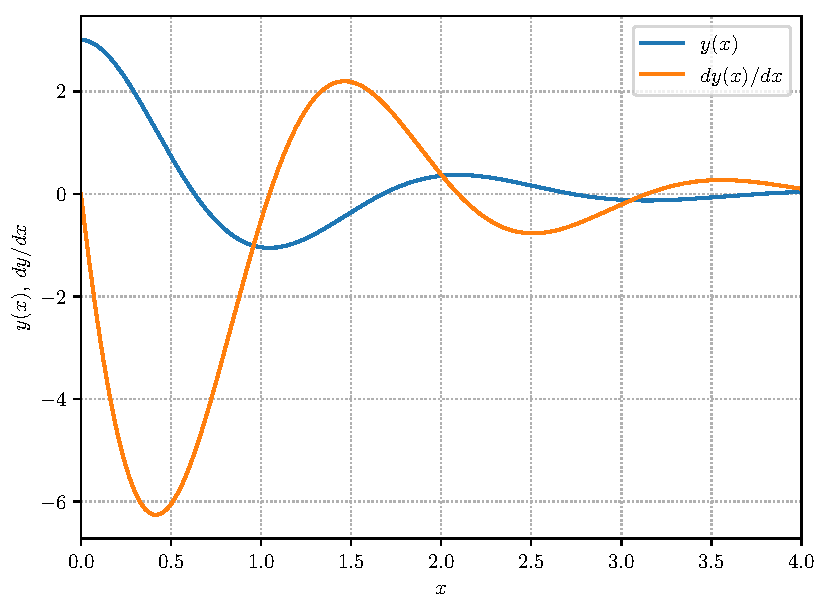
\includegraphics[width=0.75\textwidth]{mixed-fig.pdf}}{Failed to create pdf plot.}
   \captionof{figure}{The function and its derivative.}
\end{minipage}

\end{document}
